\documentclass[12pt]{article}
\usepackage[a4paper, total={7.5in, 11in}]{geometry}
\usepackage{graphicx, subfig, wrapfig, fancyhdr, lastpage, multicol ,color,arydshln,makecell, mhchem}
\usepackage[mathscr]{euscript}
\usepackage{tabularray}

\newcommand\headerMe[2]{\noindent{}#1\hfill#2}

\setlength{\columnseprule}{1pt}
\def\columnseprulecolor{\color{blue}}


\pagestyle{fancy}
\fancyhf{}

\cfoot{ \vspace{-0.8cm}\em{Page \thepage \hspace{1pt} / \pageref{LastPage}}}
\begin{document}

\headerMe{Royaume du Maroc}{année scolaire \emph{2023-2024}}\\
\headerMe{Ministère de l'Éducation nationale, }{  Professeur :\emph{Zakaria Haouzan}}\\
\headerMe{du Préscolaire et des Sports}{Établissement : \emph{Lycée SKHOR qualifiant}}\\
\vspace{-1cm}
\begin{center}
Devoir Surveillé  N°1 \\
    2ème année baccalauréat Sciences physiques\\
Semestre 2 - Durée 2h00
\\
    \vspace{.2cm}
\hrulefill
\Large{Chimie 7pts - 42min}
\hrulefill\\

    %\emph{Les deux parties sont indépendantes}
\end{center}
%end Headerss------------------------
%__________________Chimie ______________________-
%%%%%%%+_+_+_+_+_+_+_+_+_Partie1
%\vspace{-1cm}

L’acide éthanoïque pur de formule brute $CH_3COOH$, est un liquide incolore,
inflammable. Il est naturellement présent dans le vinaigre. C’est un antiseptique et un
désinfectant.
Cet exercice vise :
\begin{itemize}
	\item  L’étude d’une solution aqueuse d’acide éthanoïque,
	\item  Dosage d’une solution aqueuse d’acide éthanoïque.
\end{itemize}
 \section*{Partie1 : Etude d’une solution aqueuse d’acide éthanoïque  \dotfill(7 pts) }

On dispose d’une solution aqueuse (S) d’acide éthanoïque CH3COOH de volume
$V= 500mL$ , de concentration molaire $C_A = 5.10^{-2} mol/L$ et de $pH=3,05$.

\textbf{Données : } 
\begin{itemize}
	\item Toutes les mesures sont effectuées à 25°C.
	\item Le produit ionique de l’eau : $K_e = 10^{-14}$.
\end{itemize}

\begin{tabular}{c|l}
	0,5  & \makecell[l]{ \textbf{1.1. }Ecrire l’équation modélisant la transformation chimique entre l’acide éthanoïque
et l’eau. }\\
	1  & \makecell[l]{ \textbf{1.2. }Calculer la valeur du taux d’avancement final $\tau$ de cette réaction. Conclure. }\\
	0,5  & \makecell[l]{ \textbf{1.3. } Déterminer la constante d’équilibre K de cette réaction.}\\
	1 & \makecell[l]{ \textbf{1.4. }Déterminer la constante  $pK_A$ du couple ${CH_3COOH}_{(aq)}/{CH_3COO^-}_{(aq)}$ }\\ 
	0,5 & \makecell[l]{ \textbf{1.5. }Dresser le diagramme de prédominance et déduire l’espèce prédominante }\\ 
	\end{tabular}

 \section*{Partie 2 : Dosage d’une solution aqueuse d’acide éthanoïque.\dotfill}
Pour vérifier la valeur de la concentration molaire CA de la solution (S), on dose un
volume $V_A$=$25,0mL$ par une solution aqueuse $(S_B)$ d’hydroxyde de sodium ($Na^+_{(aq)} + HO^-_{(aq)}$) de concentration molaire \\$C_B $=$6,25.10^{-2}mol/L$. Pour cela on utilise un montage de
dosage pH-métrique. Le volume versé de la solution (SB) à l’équivalence est $V_{BE} = 20,0mL$.

\begin{tabular}{c|l}
	1  & \makecell[l]{ \textbf{2.1. }Faire un schéma légendé du montage expérimental utilisé.}\\
	0,5  & \makecell[l]{ \textbf{2.2. }Ecrire l’équation chimique modélisant la réaction du dosage.}\\
	1  & \makecell[l]{ \textbf{2.3 }Choisir l’affirmation juste parmi les affirmations suivantes:
\\À l’équivalence d’un titrage acido-basique:\\ 
 a- le volume du réactif titrant est toujours égal à celui du réactif titré.\\
b- le pH du mélange réactionnel est toujours égal à 7.\\
c- les quantités de matière des réactifs sont nulles.\\
d- le réactif titré n’a pas totalement réagi.\\
	}\\
	0,5  & \makecell[l]{ \textbf{2.4 }la valeur de CA est-elle vérifiée? Justifier la réponse.}\\
	0,5  & \makecell[l]{ \textbf{2.5 }Déterminer le pH du mélange réactionnel quand on a versé le volume: $V_B = \frac{2}{3}.V_{BE}$ }\\
	\end{tabular}
%\hrulefill
%\Large{Physique 13pts/78min}
%\hrulefill\\
%	\vspace{3cm}
\begin{center}
    %\vspace{.60cm}
\hrulefill
\Large{Physique 13pts - 78min}
\hrulefill\\
    \emph{Les  parties sont indépendantes}
\end{center}

\section*{Partie 1 : Réponse d’un dipôle RC à un échelon de tension\dotfill(3,5pts)}
\begin{wrapfigure}[9]{r}{0.3\textwidth}
\vspace{-1.2cm}
\begin{center}
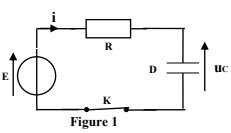
\includegraphics[width=0.3\textwidth]{./Rc00.png}
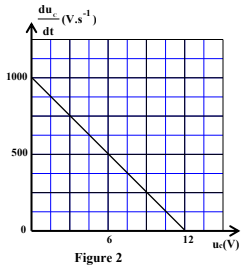
\includegraphics[width=0.3\textwidth]{./rc01.png}
\end{center}
\end{wrapfigure}


On réalise le montage, représenté sur le schéma de
la figure 1, constitué des éléments suivants :
\begin{itemize}
	\item Un générateur idéal de tension de force électromotrice E
	\item Un condensateur D de capacité C initialement déchargé
	\item Un conducteur ohmique de résistance $R = 10^3\Omega$.
	\item Un interrupteur K.

\end{itemize}
On ferme l’interrupteur à un instant choisi comme origine des
dates t = 0. Un système d’acquisition informatisé permet de
tracer la courbe de la figure 2, représentant les variations de $\frac{du_c}{dt}$
en fonction de $u_c$. 
$u_c$ étant la tension à un instant t.

\begin{tabular}{c|l}
	0,25 & \makecell[l]{ \textbf{1.1. }Montrer que l’équation différentielle vérifiée par la tension $u_c(t)$.} \\
	0,5 & \makecell[l]{ \textbf{1.2. }Recopier le schéma du montage et représenter en convention \\récepteur les tensions $u_C$ et $u_R$.
	comment faut-il brancher un \\oscilloscope à mémoire pour visualiser la tension $u_C$} \\
	0.75 & \makecell[l]{ \textbf{1.3. }Montrer que l’intensité du courant électrique : $i(t) = \frac{E}{R}.e^{\frac{-t}{\tau}}$. } \\
	1 & \makecell[l]{ \textbf{1.4. }En se basant sur le graphe de la figure 2
ci-contre, déterminer :la f.e.m E du générateur.\\et la constante du temps $\tau$ } \\
	1 & \makecell[l]{\textbf{1.5. }En exploitant la figure 2 , montrer que la capacité du
	\\condensateur est : $C = 12\mu F$ }\\
\end{tabular}

\section*{Partie 2 : Réponse d’un dipôle RL à un échelon de tension \dotfill(4pts) }
On réalise le montage schématisé sur la figure1.
Ce montage comporte :

\begin{center}
  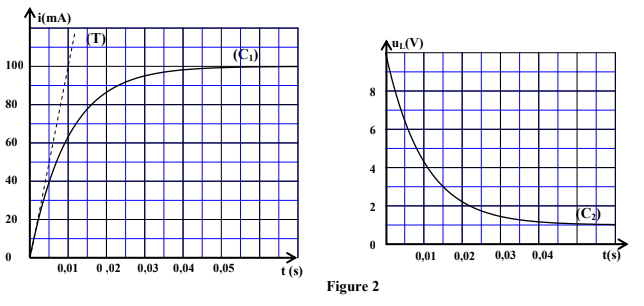
\includegraphics[width=1\textwidth]{./Rl00.png}
\end{center}

\begin{itemize}
	\item Une bobine d’inductance L et de résistance r.
	\item un conducteur ohmique de résistance $R = 90 \Omega$
	\item un générateur de force électromotrice E et de résistance
interne négligeable ;
\item un interrupteur K.
\end{itemize}
On ferme l’interrupteur à un instant de date t = 0.
Un système d’acquisition informatisé permet de tracer les courbes (C1) et (C2) représentant
successivement l’évolution de l’intensité du courant i(t) traversant le circuit et l’évolution de
la tension uL (t) aux bornes de la bobine.
La droite (T) représente la tangente à la courbe (C1) à t = 0. (figure 2).

\begin{tabular}{c|l}
	0,25 & \makecell[l]{\textbf{2.1. }Montrer que l’équation différentielle vérifiée par l’intensité du courant i(t) \\s’écrit ainsi: $\frac{di}{dt} + \frac{R + r}{L}.i = \frac{E}{L}$ }\\
	0,75	&\makecell[l]{\textbf{2.2. }En exploitant les deux courbes (C1) et (C2) , lorsque le régime permanent est atteint, \\déterminer
la valeur de r. }\\
	1,25 & \makecell[l]{\textbf{2.3. }Vérifier que L = 1H. }\\
	1,75 & \makecell[l]{\textbf{2.4. }Déterminer l’instant t auquel la bobine a stocké 75\% de son énergie maximale. }\\
\end{tabular}


\section*{Partie 3 :  Circuit RLC série. \dotfill(5.5pts)}
\vspace{-0.4cm}

\begin{wrapfigure}[1]{r}{0.25\textwidth}
	\vspace{-1.2cm}
\begin{center}
  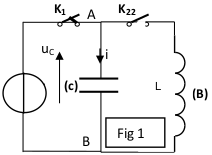
\includegraphics[width=0.25\textwidth]{./ex_011.png}
\end{center}
\end{wrapfigure}


On considère le circuit électrique schématisé dans la figure 4, comportant :

\begin{itemize}
	\item Un générateur de tension continue (G), de f.é.m $U_0$ et de résistance interne \\ négligeable, Un condensateur (c) de capacité C et d’armatures A et B \\et de charge $Q_0 = 10^{-6}C$ ;
	\item Une bobine (B) d’inductance L et de résistance négligeable ;
	\item Deux interrupteurs $K_1$ et $K_2$.

\end{itemize}




\begin{tabular}{c|l}
	0,25& \makecell[l]{\textbf{1. }$K_2$ étant ouvert, on ferme $K_1$. Après une brève durée, le condensateur porte une charge \\maximale $Q_0$
	et emmagasine une énergie électrostatique $E_0$.Donner l’expression de $Q_0$ en fonction\\ de $U_0$ et C.
et l’expression de $E_0$ en fonction de $Q_0$ et C.}\\

\end{tabular}

Le condensateur étant chargé, à t = 0 on ouvre $K_1$ et on ferme $K_2$. A t quelconque, l’armature A du
condensateur porte une charge q.

\begin{tabular}{c|l}
	0,75 & \makecell[l]{\textbf{2. }Exprimer l’énergie électromagnétique E en fonction de L, C, q et $i$.}\\

	0,75 & \makecell[l]{\textbf{3. }Montrer, sans faire aucun calcul que cette énergie se conserve et elle est égale à $\frac{Q_0^2}{2.C}$  }\\

	0,75 & \makecell[l]{\textbf{4. }Déduire l’équation différentielle des oscillations électriques régissant les variations $u_c$  }\\
	
	0,25 & \makecell[l]{\textbf{5. }Déterminer l’expression de la période propre $T_0$ en fonction de L et C.  }\\
	
\end{tabular}

Une étude expérimentale a permis de tracer les courbes (1) et (2) (ci-dessous) traduisant
respectivement les variations de l’énergie magnétique EL en fonction de i et en fonction du temps.

\begin{center}
  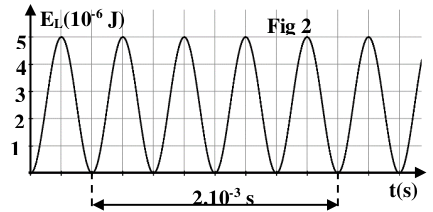
\includegraphics[width=0.5\textwidth]{./physBad.png}
\end{center}


\begin{tabular}{c|l}
	1 & \makecell[l]{\textbf{8. }Montrer que l’énergie magnétique EL est périodique de période $T = \frac{T_0}{2}$ }\\
	1,75 & \makecell[l]{\textbf{10. }déduire la valeur de $L$ et $C$ }\\


\end{tabular}



\end{document}
